% !TEX encoding = UTF-8
% !TEX TS-program = pdflatex
% !TEX root = ../tesi.tex

%**************************************************************
\chapter{Appendice A}
%**************************************************************

\section{Funzionamento di Hibernate} %TODO ORM
Come avviene la conversione delle tabelle in classi Java?\\
\begin{figure}[h]
	\centering
	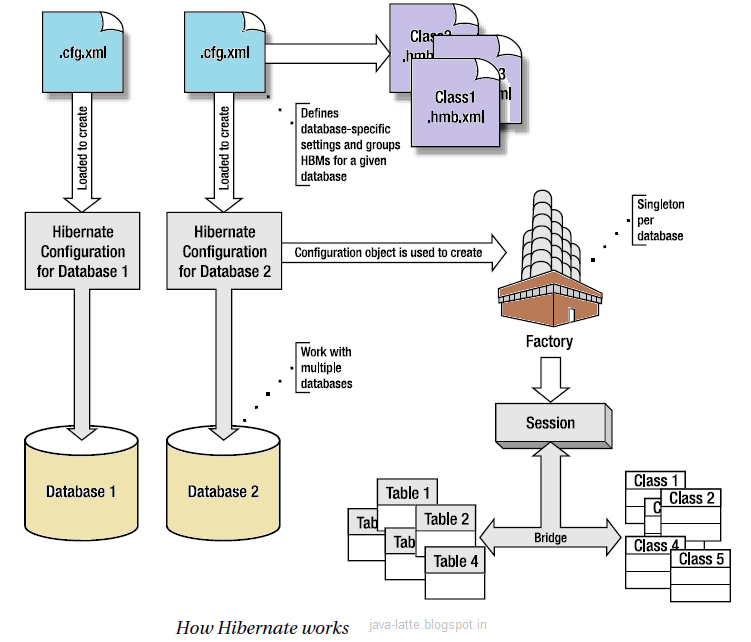
\includegraphics[height = 5 cm]{hibernate_works}
	\caption{Schema del funzionamento di Hibernate}
	\label{schema-generale}
\end{figure}
Hibernate deve conoscere la configurazione del database e per farlo necessita di un file, estesi generalmente in \textbf{.cfg.xml}. Al framework è inoltre indispensabile fornire dei files di mapping, uno per ogni tabella e generalmente estesi con i suffissi \textbf{.hmb.xml}, che contengono le informazioni riguardanti le colonne della singola tabella da trasformare in un oggetto Java.\\

\begin{figure}[h]
	\centering
	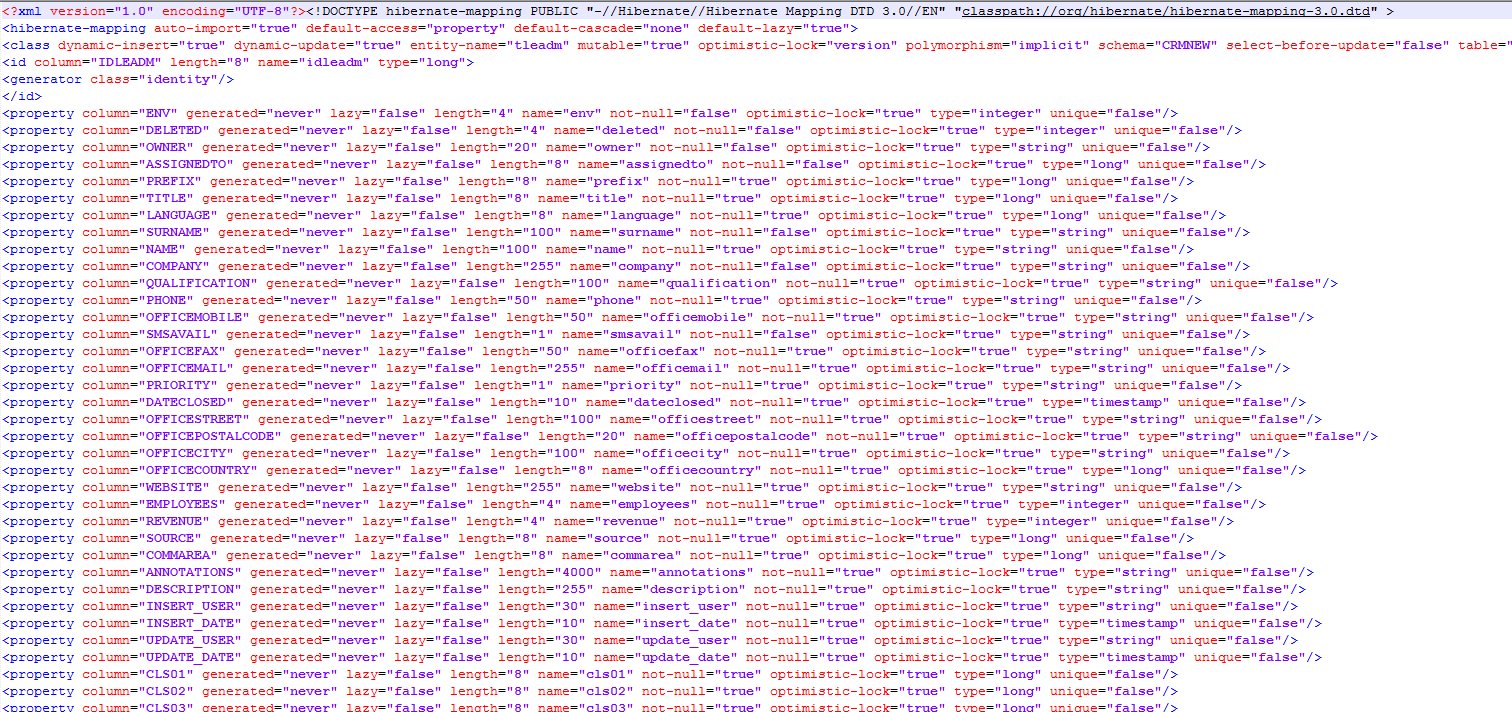
\includegraphics[height = 5 cm]{hibernate-entities}
	\caption{XML di un'entità Hibernate}
	\label{entità}
\end{figure}

Questi files vengono poi utilizzati per creare una \emph{SessionFactory} globale e thread-safe che funge da \emph{gateway} per l'interrogazione del database. \\ I vantaggi dell'utilizzo della tecnica di programmazione ORM (Object-Relational Mapping) sono molteplici ed in particolare consentono:
\begin{itemize}
	\item \textbf{Disaccoppiamento dal DBMS};
	\item \textbf{Elevata portabilità};
	\item \textbf{Drastica riduzione del codice sorgente}, a causa dei semplici comandi che mascherano complesse istruzioni;
	\item \textbf{Elevata modularità}.
\end{itemize}



